\chapter*{The IS--LM Model}
\section*{1. Standard IS-LM Framework (Upward-Sloping LM Curve)}
\begin{figure}[h!]
    \centering
    \begin{tikzpicture}[scale=1.0]
        \draw[->] (0,0) -- (5.5,0) node[right] {$Y$ (Output)};
        \draw[->] (0,0) -- (0,5.5) node[above] {$i$ (Interest Rate)};
        \draw[thick,blue] (1,4) -- (4,1) node[right] {IS};
        \draw[thick,red] (1,1) -- (4,4) node[right] {LM};
        \draw[dotted] (2.5,0) -- (2.5,2.5) -- (0,2.5);
        \draw (2.5,2.5) node[circle,fill,inner sep=1.5pt]{};
        \node[yshift=0.33cm] at (2.5,2.5) {$E$};
    \end{tikzpicture}
    \caption{A simple IS-LM diagram with an upward-sloping LM curve. 
    The intersection at $E$ represents the equilibrium in both the goods and money markets.}
\end{figure}

\noindent
\textbf{Interpretation:} 
\begin{itemize}
    \item \emph{IS line (blue)}: Shows the inverse relationship between the interest rate $i$ and output $Y$ that equilibrates the goods market (higher $i$ reduces investment and thus reduces $Y$).
    \item \emph{LM line (red)}: Reflects the positive relationship between $Y$ and $i$ in the money market (more output raises money demand, pushing up the interest rate).
    \item \emph{Equilibrium ($E$)}: Where the two lines intersect, determining the simultaneous equilibrium in both markets.
\end{itemize}

\section*{2. IS--LM Model with a Fixed Interest Rate (Horizontal LM)}
\begin{figure}[h!]
    \centering
    \begin{tikzpicture}[scale=1.0]
        \draw[->] (0,0) -- (5.5,0) node[right] {$Y$ (Output)};
        \draw[->] (0,0) -- (0,5.5) node[above] {$i$ (Interest Rate)};
        \draw[thick,blue] (1,4) -- (4,1) node[right] {IS};
        \draw[thick,red] (0.5,2.5) -- (5,2.5) node[right] {LM ($i$ fixed)};
        \draw[dotted] (2.5,0) -- (2.5,2.5) -- (0,2.5);
        \draw (2.5,2.5) node[circle,fill,inner sep=1.5pt]{};
        \node[above right] at (2.5,2.5) {$E'$};
    \end{tikzpicture}
    \caption{IS-LM diagram with a fixed interest rate. The LM curve is horizontal, 
    indicating that the central bank keeps $i$ constant regardless of output $Y$.}
\end{figure}

\noindent
\textbf{Interpretation:}
\begin{itemize}
    \item With a fixed interest rate, the LM curve becomes perfectly elastic (horizontal). 
    \item Any change in $Y$ does not affect $i$, as the central bank accommodates changes in money demand by adjusting the money supply.
    \item The new equilibrium $E'$ remains at the same interest rate but can shift in terms of output if the IS line moves (e.g., due to fiscal policy).
\end{itemize}

\section*{IS Curve Shift: Decrease in Autonomous Investment}
A decrease in autonomous investment (\(\bar{I}\)) reduces aggregate demand for any given interest rate, causing the IS curve to shift left (i.e., equilibrium output is lower at every interest rate). The magnitude of this shift depends on the relevant multiplier:
\[
\text{Multiplier} = 
\begin{cases}
\frac{1}{1-c} & \text{(Closed economy, no government)},\\[1em]
\frac{1}{1 - c(1-t)} & \text{(Closed economy, with government)},\\[1em]
\frac{1}{1 - c(1-t) + z} & \text{(Open economy, with imports)}.
\end{cases}
\]
Here, \(c\) is the marginal propensity to consume, \(t\) the net tax rate, and \(z\) the marginal propensity to import. A drop in \(\bar{I}\) therefore shifts the IS curve left by \(\Delta \bar{I}\) times the relevant multiplier.
\begin{figure}[h!]
    \centering
    \begin{tikzpicture}[scale=1.0]
        \draw[->] (0,0) -- (5.5,0) node[right] {$Y$ (Output)};
        \draw[->] (0,0) -- (0,5.5) node[above] {$i$ (Interest Rate)};
        \draw[thick,blue] (1,4) -- (4,1) node[right] {$\text{IS}_1$};
        \draw[thick,purple] (1,3) -- (3,1) node[right] {$\text{IS}_2$};
        \draw[thick,red] (1,1) -- (4,4) node[right] {LM};
        \draw[dotted] (2.5,0) -- (2.5,2.5) -- (0,2.5);
        \draw (2.5,2.5) node[circle,fill,inner sep=1.5pt]{};
        \node[xshift=0.012cm,yshift=0.37cm] at (2.5,2.5) {$E_1$};
        \draw[dotted] (2,0) -- (2,2) -- (0,2);
        \draw (2,2) node[circle,fill,inner sep=1.5pt]{};
        \node[yshift=0.37cm] at (2,2) {$E_2$};
    \end{tikzpicture}
    \caption{Leftward shift of the IS curve (\(\text{IS}_1 \to \text{IS}_2\)) due to a decrease in autonomous investment. 
    Equilibrium moves from \(E_1\) to \(E_2\), reducing both output (\(Y\)) and the interest rate (\(i\)) in this example.}
\end{figure}

\noindent
\textbf{Key Points:}
\begin{itemize}
    \item \textbf{Autonomous Investment Decreases:} For a given interest rate, firms reduce their planned investment, lowering aggregate demand.
    \item \textbf{IS Curve Shifts Left:} Equilibrium output is smaller at every interest rate.
    \item \textbf{Multiplier Effect:} The total change in output depends on how large the multiplier is, which in turn depends on the structure of the economy (presence of taxes, openness to trade, etc.).
    \item \textbf{New Equilibrium:} The economy moves from \(E_1\) to \(E_2\), where output \(Y\) is lower and, in this example, the interest rate \(i\) is also somewhat lower.
\end{itemize}

\section*{Factors Causing a Leftward Shift of the IS Curve}
\noindent
The IS curve represents equilibrium in the goods market: 
\[
Y = C + I + G + NX.
\]
A leftward shift means that, at any given interest rate $i$, the equilibrium level of output $Y$ is lower. This can result from:
\begin{itemize}
    \item \textbf{Decrease in Autonomous Consumption:}
    \begin{itemize}
        \item Households reduce their consumption due to lower consumer confidence, a negative wealth effect (e.g., a decline in stock or housing prices), or pessimistic future income expectations.
        \item This lowers aggregate demand directly.
    \end{itemize}
    \item \textbf{Decrease in Autonomous Investment:}
    \begin{itemize}
        \item Firms reduce planned investment (e.g., due to lower business confidence, less optimistic profit expectations, or stricter lending standards).
        \item This reduces aggregate demand and shifts the IS curve left.
    \end{itemize}
    \item \textbf{Decrease in Government Spending ($G$):}
    \begin{itemize}
        \item If the government cuts its expenditures (for instance, due to austerity measures or attempts to reduce budget deficits), then for any given interest rate, total planned spending is lower.
        \item The IS curve shifts left by the change in $G$ multiplied by the relevant fiscal multiplier.
    \end{itemize}
    \item \textbf{Increase in Taxes ($T$) or Net Tax Rate ($t$):}
    \begin{itemize}
        \item When households face higher taxes, their disposable income declines, leading to lower consumption.
        \item This lowers aggregate demand at each interest rate and shifts the IS curve left.
    \end{itemize}
    \item \textbf{Decrease in Net Exports ($NX$):}
    \begin{itemize}
        \item In an open economy, a drop in exports (e.g., due to a foreign recession) or a rise in imports (e.g., from an increase in the marginal propensity to import $z$) reduces net exports.
        \item The reduction in net exports shifts the IS curve left.
    \end{itemize}
    \item \textbf{Increase in the Marginal Propensity to Save:}
    \begin{itemize}
        \item If consumers decide to save more (and thus consume less) at every level of income, then autonomous consumption or overall consumption demand decreases.
        \item This effectively lowers aggregate demand, shifting IS left.
    \end{itemize}
\end{itemize}

\section*{IS Curve Rotation with a Common Horizontal Intercept}
Suppose our original IS curve is:
\[
\text{IS}_1:\quad i = 5 - Y,
\]
which intersects the vertical axis at \((0,5)\) and the horizontal axis at \((5,0)\). 
Now assume banks start charging a higher risk premium that grows with the interest rate, effectively reducing investment for a given safe rate.  Graphically, we can capture this by a “flatter” IS curve that still passes through \((5,0)\) but has a smaller (less negative) slope in \((Y,i)\)-space:
\[
\text{IS}_2:\quad i = 2.5 \;-\; 0.5\,Y.
\]
It also crosses at \((5,0)\) on the horizontal axis but now intersects the vertical axis at \((0,2.5)\).  
\begin{figure}[h!]
    \centering
    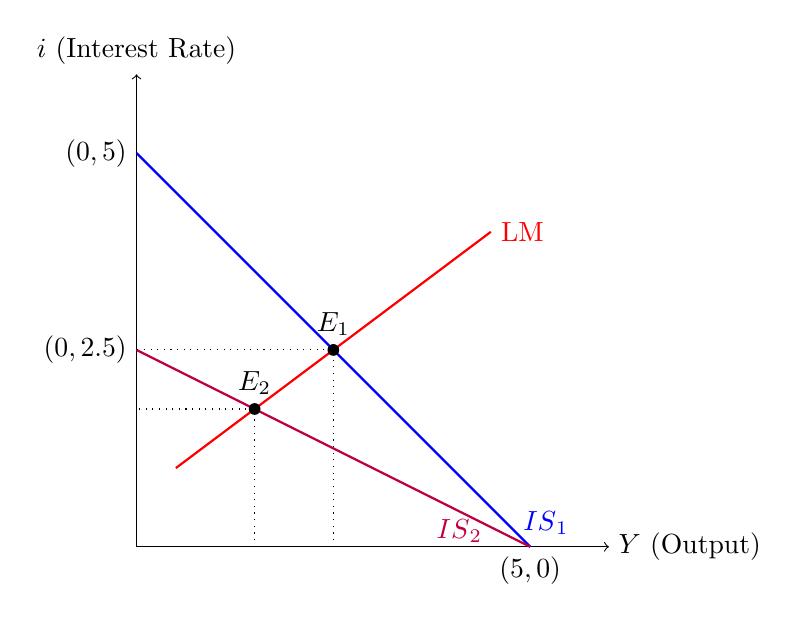
\begin{tikzpicture}[scale=1.0]
        \draw[->] (0,0) -- (6,0) node[right] {$Y$ (Output)};
        \draw[->] (0,0) -- (0,6) node[above] {$i$ (Interest Rate)};
        \draw[thick,blue] (0,5) -- (5,0) node[xshift=0.2cm, yshift=0.3cm] {$\text{IS}_1$};
        \node[left] at (0,5) {$(0,5)$};
        \node[below] at (5,0) {$(5,0)$};
        \draw[thick,purple] (0,2.5) -- (5,0) node[xshift=-0.9cm,yshift=0.2cm] {$\text{IS}_2$};
        \node[left] at (0,2.5) {$(0,2.5)$};
        \draw[thick,red] (0.5,1) -- (4.5,4) node[right] {LM};
        \draw[dotted] (2.5,0) -- (2.5,2.5) -- (0,2.5);
        \draw (2.5,2.5) node[circle,fill,inner sep=1.5pt]{};
        \node[yshift=0.33cm] at (2.5,2.5) {$E_1$};
        \draw[dotted] (1.5,0) -- (1.5,1.75) -- (0,1.75);
        \draw (1.5,1.75) node[circle,fill,inner sep=1.5pt]{};
        \node[yshift=0.33cm] at (1.5,1.75) {$E_2$};
    \end{tikzpicture}
    \caption{Both IS curves intersect at $(5,0)$, but $\text{IS}_2$ has a flatter slope 
    and intersects the vertical axis at $(0,2.5)$. 
    With an upward-sloping LM, the equilibrium shifts from $E_1$ to $E_2$, 
    showing lower output (leftward shift).}
\end{figure}
\noindent
\textbf{Interpretation:}
\begin{itemize}
    \item \(\text{IS}_1\) (\(i = 5 - Y\)) is steeper, meeting the axes at \((0,5)\) and \((5,0)\).
    \item \(\text{IS}_2\) (\(i = 2.5 - 0.5\,Y\)) is “flatter,” also crossing \((5,0)\) but hitting \((0,2.5)\) on the vertical axis.
    \item For any given interest rate \(i < 5\), the new IS curve implies a lower output \(Y\). This captures a “leftward shift” in equilibrium if the LM curve is upward sloping.
    \item \textbf{Why a leftward shift?} Because at typical policy rates below 5\%, investment is now more sensitive to risk premia, effectively reducing aggregate demand for the same safe interest rate.
\end{itemize}
\noindent
\textbf{Factors that Could Produce This Shift/Rotation:}
\begin{itemize}
    \item \emph{Higher Risk Premiums} (banks charge more when policy rates rise).
    \item \emph{Stricter Lending Standards} (reducing investment at any given policy rate).
    \item \emph{Regulatory Changes} that increase banks’ cost of lending, passed on to borrowers.
    \item \emph{Increased Uncertainty} or \emph{Worse Credit Quality} among firms and households.
\end{itemize}